\chapter{Effectuer un état de l'existant}

Le projet du CCeH compte intégrer l’ensemble des documents ayant trait au schisme alexandrin ainsi que les données des différents projets numériques pouvant témoigner de cette période. Après l’identification des différents acteurs du contexte historique nous intéressant et l’ensemble documentaire à étudier, il est nécessaire de faire un état des projets numériques déjà existants. L’objectif est d’évaluer l’intérêt des données présentées ainsi que les technologies utilisées. Ce travail permet également de réfléchir au modèle de données souhaité. 


    \section{Deux projets de référence}

    \subsection{Le \textit{RI Online}}

Grâce à un projet financé par la \textit{Deutsche Forschungsgemeinschaft}\footnote{Fondation allemande pour la recherche}, les \textit{Regesta Imperii} ont été entièrement numérisés par l’Académie des Sciences et des Lettres de Mayence et la \textit{Bayerische Staatsbibliothek}\footnote{Bibliothèque d’Etat de Bavières.} entre 2001 et 2006 \footnote{Kuczera Andreas, Graphentechnologien in den digitalen Geisteswissenschaften https://kuczera.github.io/Graphentechnologien/ }. Les regesten sont accessibles en ligne sur le site internet RI Online.
Grâce à un portail de recherche, le site permet d’accéder à l’ensemble des 140.000 regesten, stockés dans une base de données MySQL classés principalement par famille puis par empereur. En plus de la consultation des regesten, il est également possible d’accéder aux sources documentaires grâce au RI OPAC, un portail de littérature médiévale en libre accès.
Le RI Online met à disposition les regesten au format HTML ou XML, plus précisément XML-CEI. L’encodage \textit{Charters Encoding Initiative} (CEI) fut créé en 2004 par un groupe de travail formé à Munich. Ce type de schéma XML est utilisé spécifiquement pour encoder les chartes médiévales. Le RI Online exploite abondamment le standard CEI et est ainsi considéré comme une référence en la matière. Sa plateforme permet notamment d’accéder aux regesten, à la documentation ou à de nombreux liens externes vers d’autres ressources ( par exemple vers le site monasterium.net). Le RI Online dispose aussi d’autres fonctionnalités dont pourrait  s’inspirer le projet du schisme alexandrin. Par exemple, l’IHM (Interface Homme-Machine)  de présentation de documents,  la structure  du schéma CEI, ou  l’API REST permettant la communication des données. 
Certains aspects pourraient néanmoins être améliorés, comme la présentation des descriptions de sources et de la littérature, qui ne sont malheureusement pas structurées, ou les URI vers les fichiers qui sont difficiles d’accès. 


\begin{figure}[h]
%centrer l'image
    \centering
    %commande qui permet de charger une image
    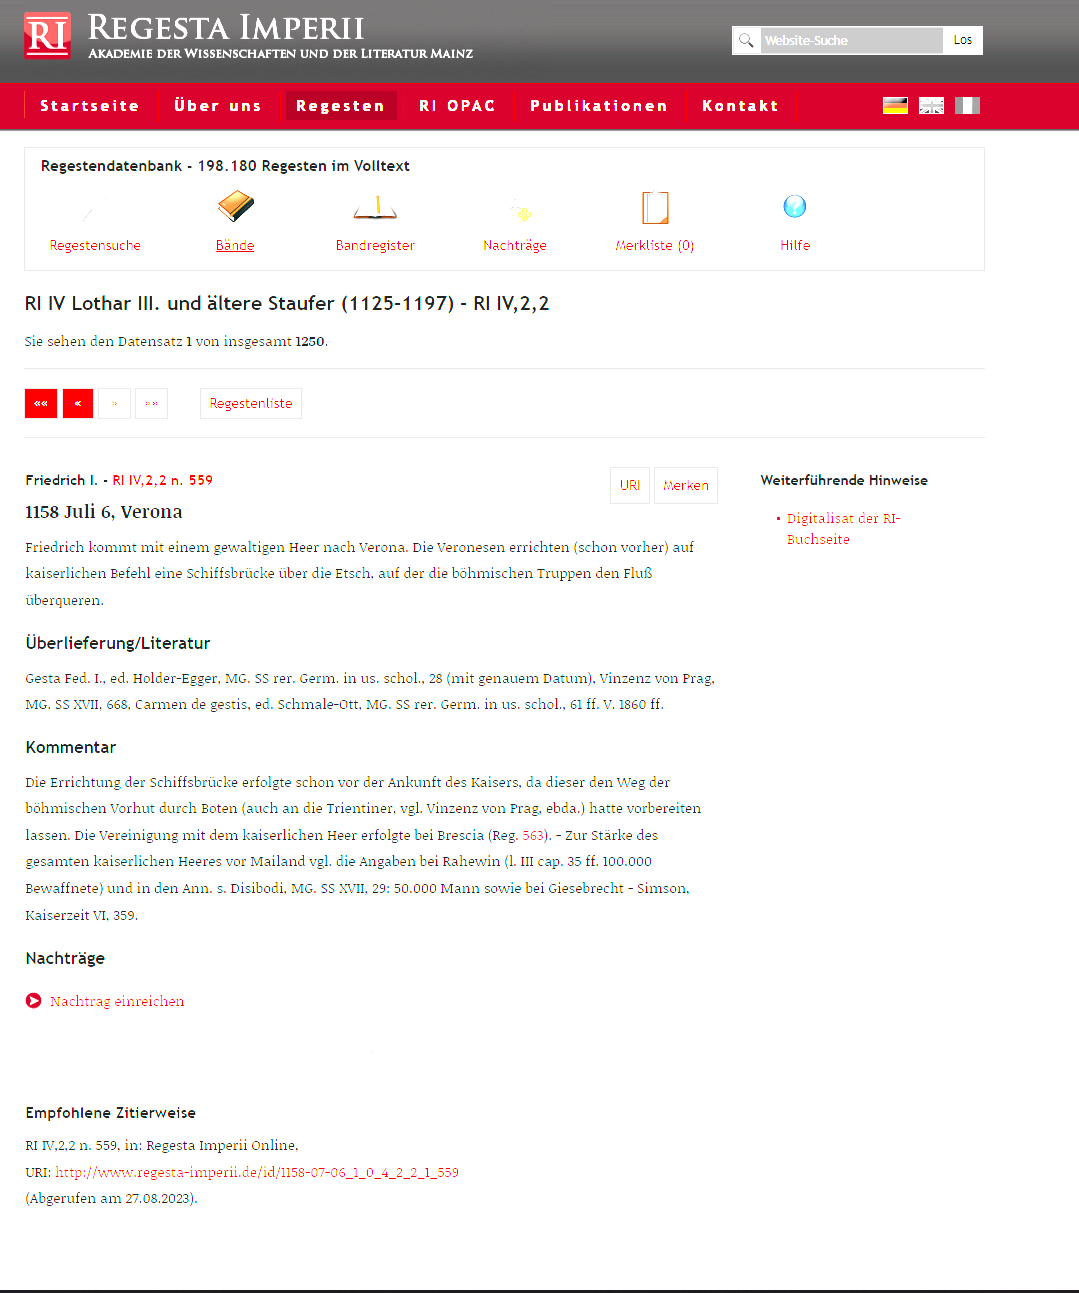
\includegraphics[width=12cm]{images/RI_online.png}
    %légende
    \caption{Capture d'écran du site RI Online, Friedrich I, RI IV,2,2 n. 559}
    %label
    \label{fig:RIonline}
\end{figure}


    \subsection{Le \textit{Papsturkunden}}

Le \textit{papsturkunden} est une collection d'éditions critiques des actes pontificaux jusqu’à Innocent III (1198), menée par la Société des sciences de Göttingen à partir du début du 20ème siècle. Cette édition est composée de répertoires nationaux, le premier étant l'Italia Pontificia entre 1906 et 1975, puis le German Pontificia à partir de 1910, et enfin le Gallia Pontificia sous la direction de l'Institut Historique Allemand (IHA) et l'École Nationale des Chartes\footnote{Hayez, M. (1999), \textit{Gallia pontificia: Répertoire des documents concernant les relations entre la papauté et les églises et monastères en france avant 1198, vol I: Diocèse de Besançon}, par B. de vregille, R. locatelli, G. Moyse et D. lohrmann (book review), Revue d'Histoire Ecclésiastique, 94(3), 927. Retrieved from https://www.proquest.com/scholarly-journals/gallia-pontificia-répertoire-des-documents/docview/1302396270/se-2}. Celui-ci est la suite des travaux de publication du \textit{Papsturkunden in Frankreich}. L'objectif est de réunir sous forme de \textit{regeste} les lettres, actes et autres documents papaux témoignant des contacts entre l’église française et la papauté. 
Entre 2007 et 2022, la Société des Sciences de Gottingen a mené un projet de base de données réunissant les différents répertoires, et en parallèle l'IHA a créé sa plateforme en ligne pour le Gallia Pontificia. Comme pour le RI Online, les bases de données du Papsturkunden et du Gallia Pontificia présentent des avantages qui pourraient être intégrés au projet. Leur principal intérêt est le format de présentation de données, principalement inspiré du Jaffé 2. Par ailleurs, plusieurs liens sont faits entre Jaffé 2 et les documents papaux grâce à l’accès au format PDF du Jaffé et de la cote donnée au document. Jaffé servant de base de référence pour une majorité des documents intégrés au projet, il est nécessaire de toujours proposer le numéro d’entrée du Regesta Pontificum Romanorum. 


\begin{figure}[h]
%centrer l'image
    \centering
    %commande qui permet de charger une image
    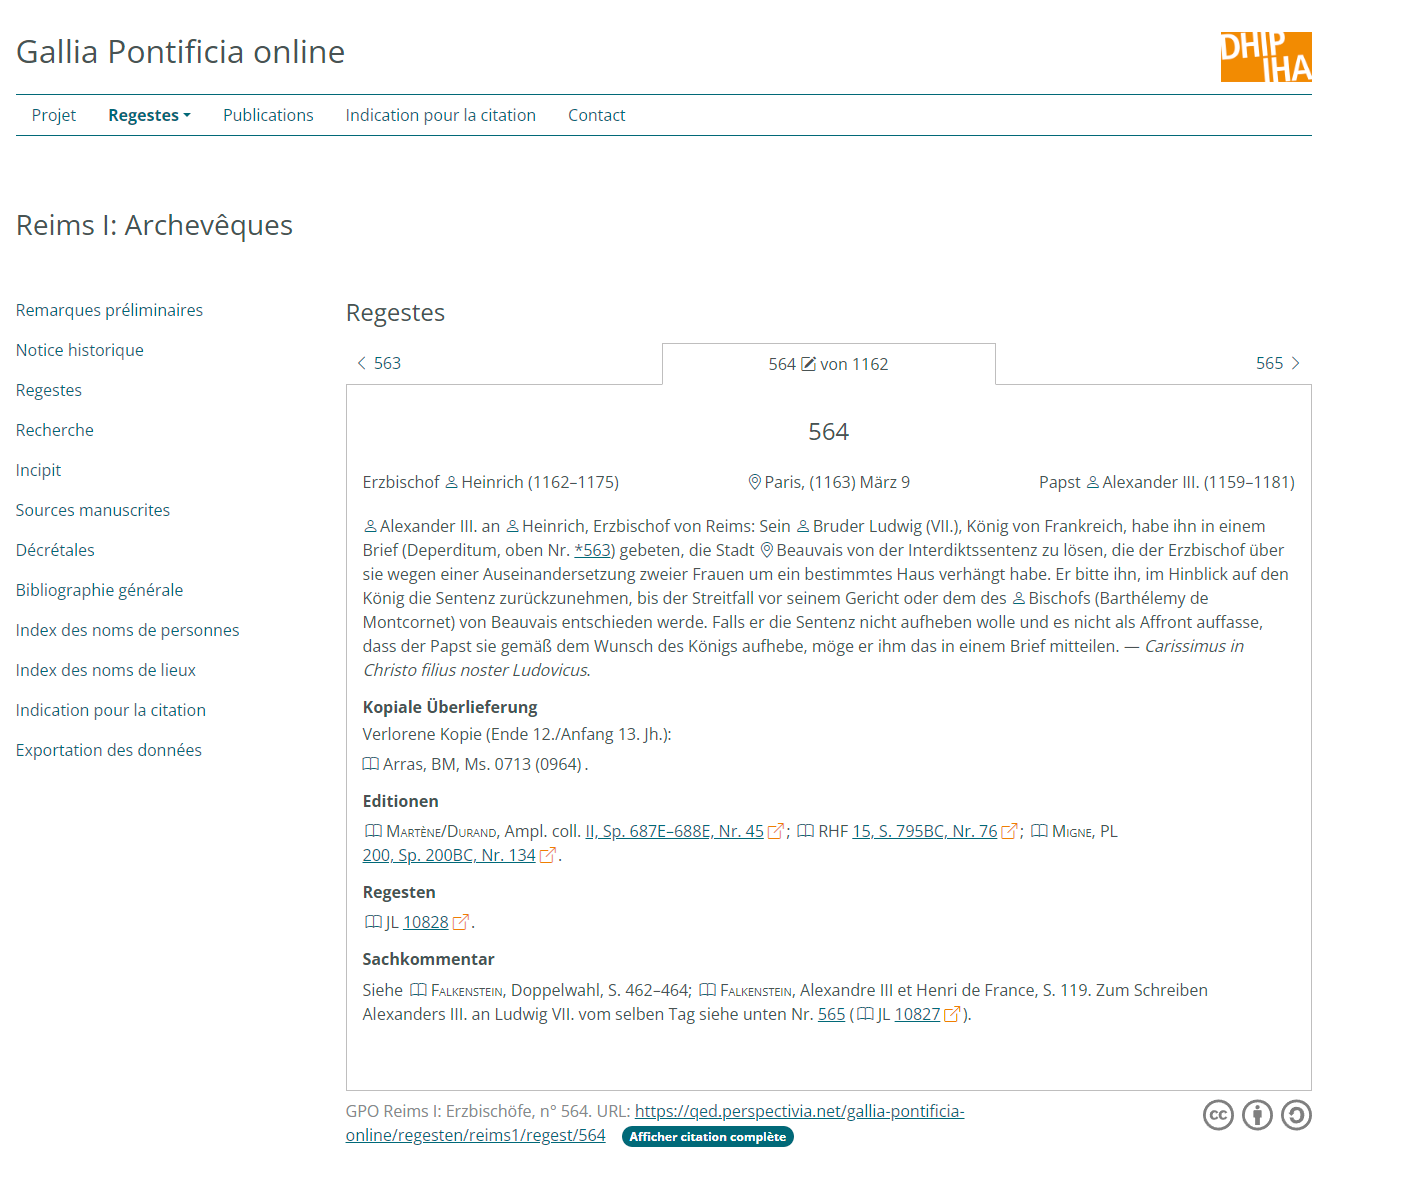
\includegraphics[width=12cm]{images/Gallia_pontificia.png}
    %légende
    \caption{Capture d'écran du site Gallia Pontificia online, regeste n°564}
    %label
    \label{fig:galliapontificia}
\end{figure}


    \section{Des bases de données déjà existantes}

Dans ce travail d’état des lieux des projets existant, on note que les documents papaux sont éparpillés entre plusieurs pays, il est donc nécessaire de s’intéresser à des projets hors du contexte allemand.\\ 
Un des principaux projets les plus intéressants et les plus importants en termes de quantités de données est la base de données française \href{http://telma-chartes.irht.cnrs.fr/}{APOSCRIPTA}, fusionnée récemment avec la base de données Chartae Galliae. Son objectif est de “rassembler les textes et métadonnées du plus grand nombre possible de documents (lettres principalement) émis par les pontifes romains depuis les origines jusqu'à l'âge moderne, quelles que soient leurs traditions manuscrites.” Cette base de données a été lancée en 2017 à l’initiative de plusieurs groupes de recherche, dont \href{https://fulmen.hypotheses.org/category/fulmen-un-programme-de-recherches-collectives}{FULMEN}\footnote{Programme international de recherche qui réunit des historiens de toutes les périodes pour des recherches sur la forme et les usages des censures canoniques de l’Antiquité tardive à nos jours.} et l’université de Lyon II. Elle permet notamment de compléter les données du \textit{papsturkunden} et \textit{Gallia Pontificia}. On compte environ 739 entrées pour le mot clef “Alexandre III”. Les éléments de description du document sont très complets, on retrouve notamment le destinataire, les dates, le lieu, le type de document, l’analyse, parfois la transcription, le numéro Jaffé, la bibliographie.\\

\begin{figure}[h]
%centrer l'image
    \centering
    %commande qui permet de charger une image
    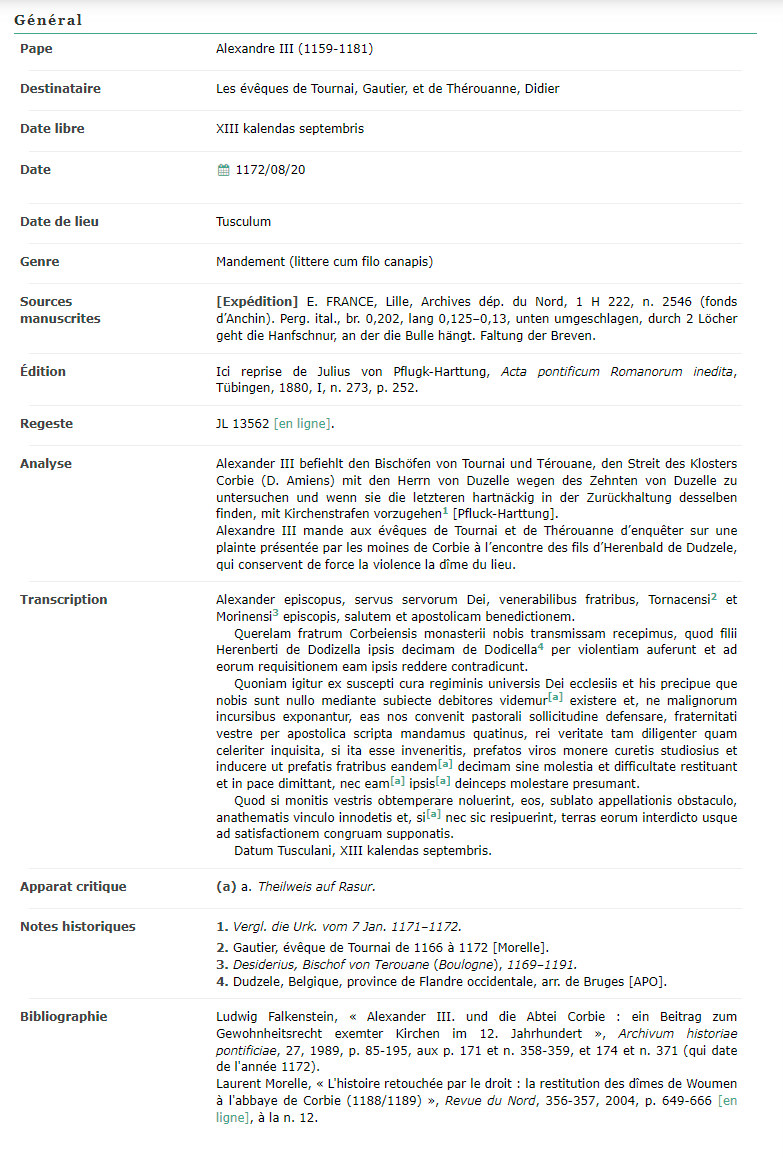
\includegraphics[width=12cm]{images/aposcripta-3461.png}
    %légende
    \caption{Capture d'écran du site APOSCRIPTA, aposcripta-3461}
    %label
    \label{fig:Aposcripta}
\end{figure}


\noindent D'autres projets intéressent les chercheurs du projet du CCeH: 
\begin{itemize}
    \item \href{https://www.diplomata-belgica.be/colophon_fr.html}{Diplomata Belgica}. Initié au milieu des années 1980, ce projet s'appuie sur une base de données réunissant environ 35000 actes expédiés des Pays-Bas méridionaux durant le Moyen-Age. Pour l'entrée "Alexandre III", on compte 483 entrées environ pour Alexandre III. Par ailleurs, le Diplomata Belgica possèdent des bonnes métadonnées et des bonnes fonctions de recherche.
    \item \href{https://deeds.library.utoronto.ca/}{Documents of Early England Data Set} (DEEDS). Ce projet fut initié en 1975 à l'université de Toronto.  inspiration pour la géolocalisation.\\
    
\end{itemize}


Prendre connaissance des données et projets déjà existants -  qui couvrent tout ou une partie du périmètre fonctionnel étudié - est une étape primordiale dans la modélisation de données. L’adoption du projet, la familiarité qu’auront les chercheurs à utiliser l’outil développé dépendra de la bonne intégration des modèles pré-existants dans le modèle conçu.
Par exemple, si l’outil développé présentait une lettre pontificale sans faire mention de son numéro Jaffé, le chercheur serait alors bien plus réticent à l’utiliser, pourrait douter de la qualité de l’outil mis entre ses mains, et finirait sans doute par le disqualifier.
C’est pourquoi, une fois l’état des lieux réalisé, il est nécessaire de mettre en place les moyens pour récupérer et intégrer les données existantes dans le projet.


